\chapter{System Design \& Implementation}
\label{ch:design-implementation}
This chapter describes the design and implementation of the core Iteration 2 modules: LLM integration, RAG pipeline, and price prediction.
\section{LLM/Policy Module}

\subsection{Architecture Overview}

The LLM module provides a unified interface for dialogue generation, supporting multiple backends for flexibility between cloud and local deployment:

\begin{enumerate}
    \item \textbf{Gemini Flash}: Google's Gemini 2.0 Flash model via the \texttt{google-generativeai} SDK for high-quality cloud inference
    \item \textbf{HuggingFace Transformers}: Local models with 4-bit/8-bit quantization for on-premise deployment
    \item \textbf{llama.cpp}: GGUF models for CPU-efficient inference without GPU requirements
\end{enumerate}

The backend selection is controlled via environment variables, with automatic detection based on model file extensions. When a GGUF file is specified, the system automatically uses llama.cpp; otherwise, it defaults to HuggingFace Transformers.

\subsection{System Prompts}

The LLM is configured with domain-specific system prompts that enforce the real estate agent persona. The prompts are designed for both Urdu and English, with explicit instructions to:

\begin{itemize}
    \item Understand client needs (budget, location, property type)
    \item Suggest suitable properties from the RAG knowledge base
    \item Provide accurate price information
    \item Maintain a polite, professional tone suitable for voice conversation
    \item Keep responses concise for natural dialogue flow
\end{itemize}

The system prompt also includes safety guidelines to prevent the agent from providing incorrect information or making commitments beyond its scope.

\subsection{Streaming Response Generation}

The dialogue API uses NDJSON (Newline-Delimited JSON) streaming for real-time token delivery. This approach provides several advantages:

\begin{itemize}
    \item \textbf{Low Latency}: Users see responses as they are generated, improving perceived responsiveness
    \item \textbf{Action Dispatch}: The stream can include action payloads to trigger UI widgets
    \item \textbf{Error Handling}: Errors can be communicated mid-stream without breaking the connection
\end{itemize}

Each streamed message follows the format: \texttt{\{"type": "token", "content": "..."\}} for text tokens, or \texttt{\{"type": "action", "data": \{...\}\}} for UI actions.

\subsection{Implementation Summary}

\begin{table}[!htbp]
\centering
\caption{LLM Module Implementation Files}
\label{tab:llm-files}
\begin{tabular}{|l|l|c|}
\hline
\textbf{File} & \textbf{Purpose} & \textbf{LOC} \\ \hline
\texttt{llm\_gemini.py} & Gemini Flash integration & 149 \\ \hline
\texttt{llm\_hf.py} & HuggingFace/llama.cpp backend & 357 \\ \hline
\texttt{\_\_init\_\_.py} & Factory functions and exports & 45 \\ \hline
\end{tabular}
\end{table}

%----------------------------------------------------------------------
\section{RAG Pipeline}

\subsection{Architecture Overview}

The Retrieval-Augmented Generation (RAG) pipeline grounds LLM responses in actual property data, ensuring accurate and verifiable information. Figure~\ref{fig:rag-arch} illustrates the pipeline architecture.


\begin{figure}
    \centering
    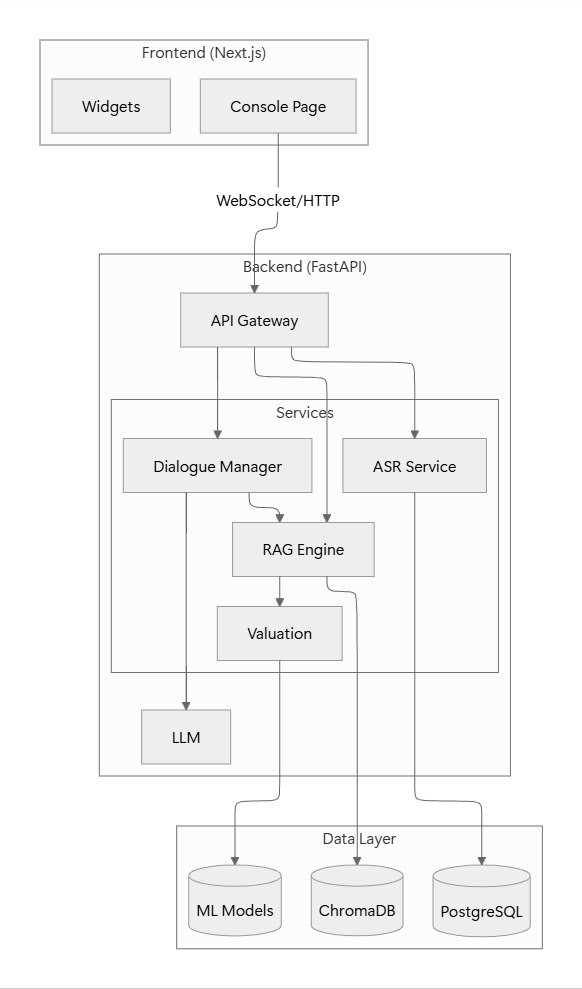
\includegraphics[width=0.75\linewidth]{ThesisFigs/High-Level_Architecture.png}
    \caption{RAG Pipeline Architecture showing data ingestion, vector indexing, and query flow}
    \label{fig:rag-arch}
\end{figure}


\subsection{Data Ingestion}

The ingestion pipeline processes multiple property datasets from various sources:

\begin{enumerate}
    \item \textbf{Dataset Loading}: CSV files from Kaggle datasets are loaded from the \texttt{data/rag/} directory
    \item \textbf{Schema Unification}: A mapping layer handles diverse column naming conventions across datasets (e.g., ``Bedrooms'' vs ``beds'' vs ``Beds'')
    \item \textbf{URL Scraping} (Optional): Full property descriptions can be fetched from Zameen.com URLs
    \item \textbf{JSONL Export}: Normalized corpus is output to \texttt{data/processed/rag\_corpus.jsonl}
\end{enumerate}

The schema unifier handles variations in column names automatically, extracting standardized fields for City, Location, Property Type, Price, Bedrooms, Baths, Area, and Description.

\subsection{Vector Store Configuration}

The system uses ChromaDB as the vector store with the following configuration:

\begin{table}[!htbp]
\centering
\caption{Vector Store Configuration}
\label{tab:vector-config}
\begin{tabular}{|l|l|}
\hline
\textbf{Parameter} & \textbf{Value} \\ \hline
Embedding Model & \texttt{paraphrase-multilingual-MiniLM-L12-v2} \\ \hline
Dimensions & 384 \\ \hline
Distance Metric & Cosine Similarity \\ \hline
Persist Directory & \texttt{data/vector/chroma} \\ \hline
Collection Name & \texttt{properties} \\ \hline
Batch Size & 512 documents \\ \hline
\end{tabular}
\end{table}

The multilingual embedding model supports 50+ languages including Urdu, enabling semantic search across both Urdu and English property descriptions.

\subsection{Query Interface}

The RAG query interface supports semantic search with optional metadata filters:

\begin{lstlisting}[language=Python, caption={RAG Query Interface}, label=lst:rag-query]
def query(
    query_text: str,
    top_k: int = 5,
    filters: Optional[Dict[str, Any]] = None,
) -> List[Dict[str, Any]]:
    col = get_collection()
    where = {}
    if filters:
        if city := filters.get("city"):
            where["city"] = city
        if min_price := filters.get("min_price"):
            where["price"] = {"$gte": float(min_price)}
    
    res = col.query(
        query_texts=[query_text],
        n_results=top_k,
        where=where or None,
    )
    return res
\end{lstlisting}

%----------------------------------------------------------------------
\section{Price Prediction Agent}

\subsection{Valuation API Design}

The valuation endpoint provides price range estimates based on property features. The API accepts property characteristics and returns a predicted price range with confidence score.

Input features include: city, property type, number of bedrooms and bathrooms, area (in square feet or Marla), and optional location string for fine-grained area detection.

\subsection{Area Unit Normalization}

A critical challenge in Pakistani real estate is the variance in ``Marla'' measurement across different housing societies:

\begin{table}[!htbp]
\centering
\caption{Marla Size Variations in Pakistan}
\label{tab:marla-sizes}
\begin{tabular}{|l|c|l|}
\hline
\textbf{Context} & \textbf{Marla Size} & \textbf{Example Locations} \\ \hline
DHA/Bahria Societies & 225 sq ft & DHA Lahore, Bahria Town \\ \hline
Punjab Revenue & 272.25 sq ft & General Punjab areas \\ \hline
\end{tabular}
\end{table}

The system automatically detects the location context and applies the appropriate conversion factor when calculating area-based price estimates.

\subsection{ML Pipeline}

The price prediction system supports loading a trained scikit-learn model from \texttt{models/price\_predictor.pkl}. The model pipeline includes feature preprocessing and a regression model trained on historical property data.

When no trained model is available, a heuristic fallback provides baseline estimates using the formula:

$$\text{Price} = \max(2,500,000, \text{Area}_{\text{sqft}} \times 12,000)$$

This heuristic produces reasonable estimates with a confidence score of 0.5, indicating to users that formal model training would improve accuracy.

%----------------------------------------------------------------------
\section{Dialogue Manager API}

\subsection{Endpoint Design}

The dialogue manager exposes several REST endpoints for the frontend:

\begin{table}[!htbp]
\centering
\caption{Dialogue Manager Endpoints}
\label{tab:endpoints}
\begin{tabular}{|l|l|p{6cm}|}
\hline
\textbf{Endpoint} & \textbf{Method} & \textbf{Description} \\ \hline
\texttt{/dialogue/step} & POST & Process dialogue turn with LLM + RAG (streaming) \\ \hline
\texttt{/rag/query} & POST & Semantic search over property listings \\ \hline
\texttt{/valuation/predict} & POST & Price range estimation \\ \hline
\end{tabular}
\end{table}

\subsection{Intent Detection}

The dialogue manager classifies user intent to route queries appropriately. Intent detection uses keyword matching for both English and Roman Urdu terms:

\begin{lstlisting}[language=Python, caption={Intent Detection Algorithm}, label=lst:intent]
def _detect_intent(text: str) -> str:
    text_lower = text.lower()
    # Price inquiry keywords (English + Roman Urdu)
    if any(k in text_lower for k in ["price", "qeemat", "kitne", "cost"]):
        return "price_query"
    # Property search keywords
    elif any(k in text_lower for k in ["property", "ghar", "plot", "flat"]):
        return "property_search"
    # Booking keywords
    elif any(k in text_lower for k in ["book", "visit", "dekhna"]):
        return "booking"
    return "general"
\end{lstlisting}

\subsection{Action Dispatch}

Based on detected intent and RAG results, the dialogue manager dispatches actions to trigger appropriate UI widgets:

\begin{table}[!htbp]
\centering
\caption{Action Types and Triggers}
\label{tab:actions}
\begin{tabular}{|l|l|l|}
\hline
\textbf{Action Type} & \textbf{Trigger} & \textbf{UI Widget} \\ \hline
\texttt{show\_price} & Price query detected & Price estimation card \\ \hline
\texttt{show\_listings} & Property search with results & Property cards grid \\ \hline
\texttt{book\_visit} & Booking intent & Appointment form \\ \hline
\end{tabular}
\end{table}

%----------------------------------------------------------------------
\section{Frontend Integration}

The Next.js frontend provides a real-time console interface for voice agent interaction. Key features include:

\begin{itemize}
    \item \textbf{Real-time Audio Streaming}: PCM audio capture using Web Audio API at 16kHz sample rate
    \item \textbf{WebSocket Communication}: Bi-directional streaming for audio and transcripts
    \item \textbf{Streaming Response Display}: Token-by-token LLM response rendering
    \item \textbf{Dynamic Widgets}: Price estimation and property listing cards triggered by actions
    \item \textbf{Waveform Visualization}: Real-time audio level display using AnalyserNode
\end{itemize}

The frontend implementation prioritizes low latency by using raw PCM streaming instead of compressed audio formats, and ScriptProcessor nodes for direct audio buffer access.